\subsubsection{Fixing $a_L = a_R = b_L = b_R = 1$}

If you compare the functions in the cobwebs \Crefrange{fig:quad.full.CobwebA}{fig:quad.full.CobwebB} to the functions of the original model in \Crefrange{fig:yunus.2pi.CobwebA2}{fig:yunus.2pi.CobwebD2} you can see some differences.
One is, that the right end of the branches $\B$ and $\D$ is higher than the left part.
To get our model to look a little more like the original model, we now skew the branches by fixing also $b_L = b_R = 1$

The 2D scan for the periods when varying $c_L$ and $c_R$ now looks different.
\Cref{fig:quadratic.full.skew.2d.full} shows the full scan, while \Cref{fig:quadratic.full.skew.2d.z1} shows an enhanced version of it, depicting the artefact in the middle of the left half of the full scan.

\begin{figure}
    \centering
    \begin{subfigure}{0.4\textwidth}
        \centering
        \includegraphics[width=\textwidth]{21_Quadratic_mod6/Skew/2D_Period_SFull/result.png}
        \caption{Full}
        \label{fig:quadratic.full.skew.2d.full}
    \end{subfigure}
    \begin{subfigure}{0.4\textwidth}
        \centering
        \includegraphics[width=\textwidth]{21_Quadratic_mod6/Skew/2D_Period_SZoomed1/result.png}
        \caption{Zoomed}
        \label{fig:quadratic.full.skew.2d.z1}
    \end{subfigure}
    \caption{2D Scan of Full Skewed Quadratic Model}
\end{figure}

\todo{replace with new cobwebs}


\begin{figure}
    \centering
    \begin{subfigure}{0.3\textwidth}
        \centering
        \includegraphics[width=\textwidth]{21_Quadratic_mod6/Cobweb_A/result.png}
        \caption{Before border}
        \label{fig:quad.full.skew.CobwebA}
    \end{subfigure}
    \begin{subfigure}{0.3\textwidth}
        \centering
        \includegraphics[width=\textwidth]{21_Quadratic_mod6/Cobweb_B/result.png}
        \caption{At border}
        \label{fig:quad.full.skew.CobwebB}
    \end{subfigure}
    \begin{subfigure}{0.3\textwidth}
        \centering
        \includegraphics[width=\textwidth]{21_Quadratic_mod6/Cobweb_C/result.png}
        \caption{After border}
        \label{fig:quad.full.skew.CobwebC}
    \end{subfigure}
    \caption{Cobwebs along marked line}
    \label{fig:quad.full.skew.Cobwebs}
\end{figure}
